\chapter{\selectlanguage{greek}Τεχνολογίες Υλοποίησης}

Στο κεφάλαιο αυτό θα περιγράψουμε τα εργαλεία και τις τεχνολογίες που χρησιμοποιήθηκαν για την υλοποίησή μας. \\

\section{Η γλώσσα προγραμματισμού \en {Python}}

Η γλώσσα προγραμματισμού {\en {Python}} \cite{Py02}, \cite{Py01} είναι μια γλώσσα διερμηνευόμενη και {\en {object-oriented}}. 
Η σύλληψη της {\en {Python}} έγινε στα τέλη της δεκαετίας του 1980 και η εφαρμογή της έγινε το Δεκέμβριο του 1989 από τον Ολλανδό {\en {Guido Van Rossum}}, 
ο οποίος είναι και ο κύριος συγγραφέας της. Το όνομα της γλώσσας προέρχεται από την ομάδα Άγγλων κωμικών {\en {Monty Python}}.
O κώδικάς της διανέμεται με την άδεια {\en {Python Software Foundation}}. 
Ανάμεσα στα κύρια χαρακτηριστικά της είναι τα εξής: γλώσσα ανοιχτού κώδικα {\en {(open source)}}, αναγνωσιμότητα, εύκολη εκμάθηση, 
επεκτασιμότητα, εύκολη συντήρηση, δυνατότητα απλοποίησης στην υλοποίηση δύσκολων συναρτήσεων, γρήγορη ανάπτυξη εφαρμογών.

\par Η ίδια η γλώσσα είναι επεκτάσιμη καθώς ένα βασικό σύνολο της γλώσσας αποτελεί τον πυρήνα της, 
ενώ όλα τα υπόλοιπα είναι βιβλιοθήκες {\en {(modules)}} που επεκτείνουν την λειτουργικότητά της. 
Oι κύριοι τύποι δεδομένων που χρησιμοποιεί είναι οι λίστες, τα λεξικά και οι πλειάδες. 
Έχει μεγαλο εύρος εφαρμογών, όπως για παράδειγμα στον επιστημονικό υπολογισμό, στην τεχνητή νοημοσύνη, 
στην επεξεργασία φυσικής γλώσσας κλπ.

\par Στην παρούσα διπλωματική εργασία χρησιμοποιήσαμε την έκδοση 3.4.0 της γλώσσας, 
η οποία σε συνδυασμό με την πλατφόρμα {\en {NLTK}} χρησιμεύουν σε πολλές εφαρμογές της επεξεργασίας φυσικής γλώσσας.

\section{\en{MySQL}}

Η {\en {MySQL}} \cite{sql01} είναι ένα ανοιχτού λογισμικού σύστημα διαχείρισης σχεσιακών βάσεων δεδομένων. 
Η ονομασία {\en {MySQL}} περιέχει δύο στοιχεία: το {\en {My}}  είναι το όνομα της κόρης του συνιδρυτή του συστήματος, {\en {Monty Widenius}} 
και το {\en {SQL}} αναφέρεται στη γλώσσα {\en {SQL (Structured Query Language)}}, 
μια γλώσσα υπολογιστών που αναπτύχθηκε ξεχωριστά από τις υλοποιήσεις συστημάτων διαχείρισης βάσεων δεδομένων 
(όπως της {\en {MySQL}}, της {\en {PostgreSQL}}, της {\en {Oracle}} κλπ).
Το πρόγραμμα τρέχει έναν εξυπηρετητή {\en {(server)}} παρέχοντας πρόσβαση πολλών χρηστών σε ένα σύνολο βάσεων δεδομένων.
Tο λογισμικό αυτό επιτρέπει στους χρήστες να δημιουργούν και να χρησιμοποιούν μια βάση δεδομένων, παρέχοντάς τους δυνατότητες όπως
ο ορισμός, η κατασκευή, η χρήση/προσπέλαση και η διαγραφή αυτής.
\par Θα μπορούσαμε να υλοποιήσουμε μια βάση δεδομένων και χωρίς τη χρήση συστήματος διαχείρισης (πχ. με χρήση αρχείων).
Τα σημαντικότερα πλεονεκτήματα του συστήματος διαχείρισης είναι η ευκολία στη σχεδίαση και την υλοποίηση, 
η γρήγορη ανάπτυξη εφαρμογών, η ακεραιότητα των δεδομένων, ο έλεγχος πρόσβασης χρηστών, η ταυτόχρονη χρήση από πολλούς χρήστες, 
ο έλεγχος ορθότητας/πλεονασμών και οι έτοιμες συναρτήσεις/αλγόριθμοι.

\par Η {\en {MySQL}} χρησιμοποιείται ευραίως σε διάφορες εφαρμογές όπως οι {\en {TYPO3, Joomla, Wordpress, phpBB, MyBB, Drupal}}.
Χρησιμοποιείται επίσης και σε κάποιες από τις πιο διαδεδομένες διαδικτυακές υπηρεσίες, όπως το {\en {Flickr}}, το {\en {YouTube}}, η {\en {Wikipedia}}, 
το {\en {Google}}, το {\en {Facebook}} και το {\en {Twitter}}.

\par Στην παρούσα διπλωματική εργασία χρησιμοποιήσαμε την έκδοση 5.6.33.

\section{\en{HTML}}

Η {\en{HTML}} (αρχικοποίηση του αγγλικού {\en {HyperText Markup Language}} \cite{Ht01}, ελλ. Γλώσσα Σήμανσης Υπερκειμένου) είναι η κύρια γλώσσα σήμανσης για τις ιστοσελίδες, 
και τα στοιχεία της είναι τα βασικά δομικά στοιχεία των ιστοσελίδων.

Η {\en{HTML}} γράφεται υπό μορφή στοιχείων {\en{HTML}} τα οποία αποτελούνται από ετικέτες {\en {(tags)}}, 
οι οποίες περικλείονται μέσα σε σύμβολα «μεγαλύτερο από» και «μικρότερο από», μέσα στο περιεχόμενο της ιστοσελίδας. 
Οι ετικέτες {\en{HTML}} συνήθως λειτουργούν ανά ζεύγη, 
με την πρώτη να ονομάζεται ετικέτα έναρξης και τη δεύτερη ετικέτα λήξης 
(ή σε άλλες περιπτώσεις ετικέτα ανοίγματος και ετικέτα κλεισίματος αντίστοιχα). 
Ανάμεσα στις ετικέτες οι σχεδιαστές ιστοσελίδων μπορούν να τοποθετήσουν κείμενο, πίνακες, εικόνες κλπ.

\par Ο σκοπός ενός {\en {web browser}} είναι να διαβάζει τα έγγραφα {\en{HTML}} και τα συνθέτει σε σελίδες που μπορεί κανείς να διαβάσει ή να ακούσει. 
Ο {\en {browser}} δεν εμφανίζει τις ετικέτες {\en{HTML}}, αλλά τις χρησιμοποιεί για να ερμηνεύσει το περιεχόμενο της σελίδας.

\par Τα στοιχεία της {\en{HTML}} χρησιμοποιούνται για να κτίσουν όλους τους ιστότοπους. 
Η {\en{HTML}} επιτρέπει την ενσωμάτωση εικόνων και άλλων αντικειμένων μέσα στη σελίδα 
και μπορεί να χρησιμοποιηθεί για να εμφανίσει διαδραστικές φόρμες. 
Παρέχει τις μεθόδους δημιουργίας δομημένων εγγράφων (δηλαδή εγγράφων που αποτελούνται από το περιεχόμενο που μεταφέρουν 
και από τον κώδικα μορφοποίησης του περιεχομένου) καθορίζοντας δομικά σημαντικά στοιχεία για το κείμενο, 
όπως κεφαλίδες, παραγράφους, λίστες, συνδέσμους, παραθέσεις και άλλα. 
Μπορούν, επίσης, να ενσωματώνονται σενάρια εντολών σε γλώσσες όπως η {\en {JavaScript}}, 
τα οποία επηρεάζουν τη συμπεριφορά των ιστοσελίδων {\en{HTML}}.

\par Οι {\en {Web browsers}} μπορούν επίσης να αναφέρονται σε στυλ μορφοποίησης {\en {CSS}} 
για να ορίζουν την εμφάνιση και τη διάταξη του κειμένου και του υπόλοιπου υλικού. 
Ο οργανισμός {\en {W3C}}, ο οποίος δημιουργεί και συντηρεί τα πρότυπα για την {\en{HTML}} και τα {\en {CSS}}, 
ενθαρρύνει τη χρήση των {\en {CSS}} αντί διαφόρων στοιχείων της {\en {HTML}} για σκοπούς παρουσίασης του περιεχομένου.

\section{\en{CSS}}

Η {\en {CSS (Cascading Style Sheets}} \cite{w3css} - Διαδοχικά Φύλλα Στυλ ή αλληλουχία
φύλλων στυλ) είναι μια γλώσσα υπολογιστή που ανήκει στην κατηγορία των
γλωσσών φύλλων στυλ που χρησιμοποιείται για τον έλεγχο της εμφάνισης
ενός εγγράφου που έχει γραφτεί με μια γλώσσα σήμανσης. Χρησιμοποιείται
δηλαδή για τον έλεγχο της εμφάνισης ενός εγγράφου που γράφτηκε στις
γλώσσες {\en {HTML}} και {\en {XHTML}}, δηλαδή για τον έλεγχο της εμφάνισης μιας
ιστοσελίδας και γενικότερα ενός ιστοτόπου.
Η {\en {CSS}} είναι μια γλώσσα υπολογιστή προορισμένη να αναπτύσσει στυλιστικά μια ιστοσελίδα, 
δηλαδή να διαμορφώνει περισσότερα χαρακτηριστικά, χρώμματα, στοίχιση και δίνει περισσότερες δυνατότητες σε σχέση με την {\en {html}}.
Η χρήση της {\en {CSS}} κρίνεται ως απαραίτητη για μια όμορφη και καλοσχεδιασμένη ιστοσελίδα .

\section{\en {Apache HTTP Server}}

Ο {\en {Apache HTTP Server}} \cite{Ap01}, γνωστός και απλά σαν {\en {Apache}}, είναι ένας εξυπηρετητής του παγκόσμιου ιστού {\en {(web)}}. 
Όποτε ένας χρήστης επισκέπτεται έναν ιστότοπο, το πρόγραμμα πλοήγησης {\en {(browser)}} επικοινωνεί με έναν διακομιστή {\en {(server)}} 
μέσω του πρωτοκόλλου {\en {HTTP}}, ο οποίος παράγει τις ιστοσελίδες και τις αποστέλλει στο πρόγραμμα πλοήγησης. 
Κυκλοφόρησε υπό την άδεια λογισμικού {\en {Apache}} και είναι λογισμικό ανοιχτού κώδικα.

\par Ο {\en {Apache}} χρησιμοποιείται και σε τοπικά δίκτυα σαν διακομιστής συνεργαζόμενος με συστήματα διαχείρισης Βάσης Δεδομένων, π.χ. {\en {MySQL}},
όπως και χρησιμοποιήθηκε στην παρούσα διπλωματική (έκδοση 2.4.7).

\section{\en{Flask Web Framework}}

Τα {\en {Web Frameworks} είναι σχεδιασμένα για να υποστηρίζουν την ανάπτυξη διαδικτυακών εφαρμογών. 
Κάθε εφαρμογή που απαιτεί τη χρήση βάσεων δεδομένων, φορμών, συνόδων {\en {(sessions), cookies} 
ή κάποιας απομακρυσμένης υπηρεσίας (όπως είναι το {\en {Twitter}}, το {\en {Facebook}} κλπ) θα ωφεληθεί αν υλοποιηθεί με κάποιο {\en {Framework}}.

\par Το {\en {Flask}} \cite{Fl01} είναι ένα {\en {micro web framework}} γραμμένο σε {\en {Python}}.

\section{Εργαλεία Επεξεργασίας Φυσικής Γλώσσας}

\subsection{\en {Tree Tagger}}
Ο {\en {Tree Tagger}} \cite{Tt01} είναι ένα εργαλείο που δημιουργήθηκε από τον {\en {Helmud
Schmid}} στο Ινστιτούτο για τον γλωσσικό υπολογισμό στο Πανεπιστήμιο της Στουτγκάρδης. 
Αποτελείται από ένα εργαλείο για σχολιασμό κειμένου με βάση το σε τι μέρος του λόγου αντιστοιχίζεται η κάθε λέξη,
καθώς και πληροφορία για λήμματα. Ο {\en {Tree Tagger}} δουλεύει πολύ καλά για την Αγγλική γλώσσα,
αλλά υποστηρίζει επίσης και άλλες γλώσσες όπως Ισπανικά, Γαλλικά, Ιταλικά, Ολλανδικά, Βουλγαρικά, Ρωσικά, Ελληνικά, Πορτογαλικά κ.λπ.
Ο {\en {Tree Tagger}} περιλαμβάνει κατηγορίες στις οποίες ανήκουν οι λέξεις. Οι
κατηγορίες αυτές αντιπροσωπεύουν στην ουσία τα μέρη του λόγου μιας
πρότασης. Ένα παράδειγμα μιας τέτοιας κατηγορίας είναι το NN, το οποίο
υποδηλώνει ουσιαστικό. 
Παρακάτω ακολουθεί ένας αναλυτικός πίνακας με τις κατηγορίες του {\en {Tree Tagger}} και τι σημαίνει η καθεμία.

\begin{figure}[!ht] \centering
	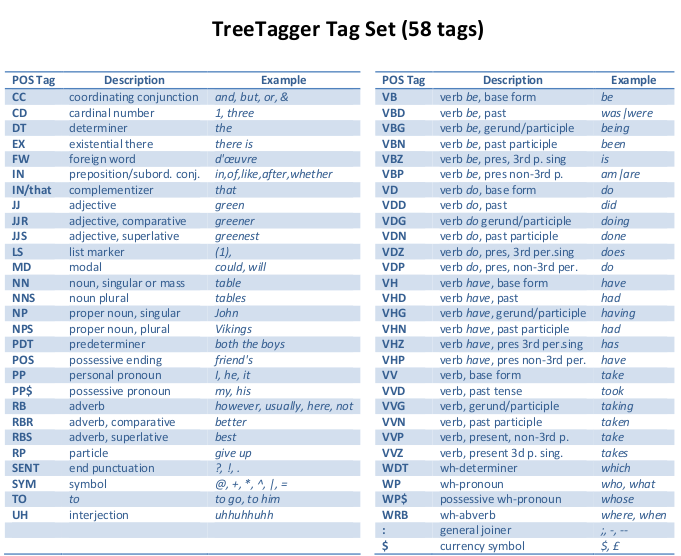
\includegraphics[scale=0.65]{static/figures/treetagger.png}
    \caption{Κατηγορίες {\en {Tree Tagger.}}}
    \label{}
\end{figure} 

\subsection{\en {NLTK}}
Το {\en {NLTK (Natural Language Toolkit)}} \cite{Nl02} είναι ένα πακέτο βιβλιοθηκών και προγραμμάτων της {\en {Python}} 
για εφαρμογές της Επεξεργασίας Φυσικής Γλώσσας και αναπτύχθηκε απ’τους
{\en {Steven  Bird,  Edward  Loper}} και {\en {Ewan  Klein}}.
Περιλαμβάνει πολλά γνωστά σώματα κειμένων, γραφικές αναπαραστάσεις
και δειγματικά δεδομένα. Συνοδεύεται από ένα βιβλίο το οποίο εξηγεί τις
έννοιες που σχετίζονται με τα εργαλεία που παρέχει. 
Βασικός στόχος του {\en {NLTK}} είναι να υποστηρίξει την έρευνα και την εκμάθηση της Επεξεργασίας
Φυσικής Γλώσσας καθώς και άλλων σχετικών πεδίων, όπως η Γλωσσολογία,
η Τεχνητή Νοημοσύνη, η Ανάκτηση Πληροφορίας και η Μηχανική Μάθηση. 
Όταν λέμε φυσική γλώσσα εννοούμε μια γλώσσα η οποία χρησιμοποιείται για την καθημερινή
επικοινωνία των ανθρώπων. Σε αντίθεση με τις τεχνητές γλώσσες, όπως οι γλώσσες προγραμματισμού
και η μαθηματική σημειογραφία, οι φυσικές γλώσσες έχουν εξελιχθεί καθώς
περνούν από γενιά σε γενιά και είναι αρκετά δύσκολο να μπορέσουν να
οριστούν με ρητούς κανόνες. 
'Εχει χρησιμοποιηθεί με επιτυχία ως εργαλείο διδασκαλίας, μελέτης και ως
πλατφόρμα για την ανάπτυξη πρωτότυπων ερευνητικών συστημάτων. \\

Το {\en {NLTK}} δημιουργήθηκε με βάση τέσσερις πρωταρχικούς σκοπούς:
\begin{itemize}
 \item \textbf{Απλότητα {\en {(Simplicity)}}}: Το να παρέχεται ένα διαισθητικό πλαίσιο εργασίας παράλληλα με ουσιώδεις
οικοδομικούς λίθους, δίνοντας στους χρήστες μια πρακτική γνώση της φυσικής επεξεργασίας γλώσσας 
χωρίς να βαλτώνουν στη βαρέτη εργασία της επεξεργασίας σχολιασμένων γλωσσικών δεδομένων.
 \item \textbf{Συνέπεια {\en {(Consistency)}}}: Το να παρέχεται ένα αμετάβλητο πλαίσιο εργασίας με συνεπείς διεπαφές και
δομές δεδομένων και εύκολα προβλέψιμα ονόματα μεθόδων.
 \item \textbf{Επεκτασιμότητα {\en {(Extensibility)}}}: Το να παρέχεται μια δομή μέσα στην οποία νέες υπομονάδες λογισμικού
μπορούν εύκολα να φιλοξενηθούν, περιλαμβάνοντας διαφορετικές υλοποιήσεις 
και περιλαμβάνοντας συναγωνιστικές προσεγγίσεις στην ίδια αποστολή.
 \item \textbf{Συναρμολογισιμότητα {\en {(Modularity)}}}: Το να παρέχονται συστατικά που μπορούν να χρησιμοποιηθούν ανεξάρτητα
χωρίς την ανάγκη κατανόησης του υπόλοιπου πακέτου.\newline
\end{itemize}

Κατά την υλοποίηση του συστήματός μας χρησιμοποιήσαμε την έκδοση 3.2.1 του {\en {NLTK}} για τις παρακάτω διαδικασίες:
\begin{itemize}
  \item \textbf{Χωρισμός του κειμένου σε προτάσεις {\en {(Sentence Tokenization/Segmentation).}}}\\
Αν θέλουμε να χωρίσουμε σε προτάσεις ένα κομμάτι κειμένου, τότε μπορούμε να ακολουθήσουμε την παρακάτω διαδικασία:
\begin{figure}[!ht] \centering
    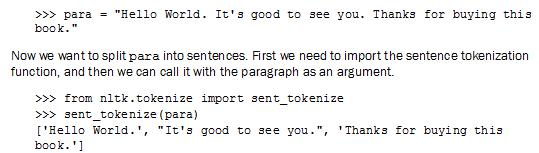
\includegraphics[scale=0.7]{static/figures/nltk1.png}
    \caption{Χωρισμός προτάσεων.}
    \label{}
\end{figure}
\\ Έτσι, τώρα έχουμε μια λίστα με τις προτάσεις και μπορούμε να τις χρησιμοποιήσουμε για περαιτέρω επεξεργασία. 

  \item \textbf{Χωρισμός των προτάσεων σε λέξεις {\en {(Word Tokenization).}}}\\
Αν θέλουμε να διαχωρίσουμε μια πρόταση σε μεμονωμένες λέξεις, θα ακολουθήσουμε τη διαδικασία που φαίνεται στην εικόνα:
\begin{figure}[!ht] \centering
    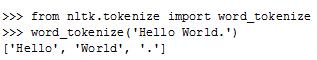
\includegraphics[scale=0.75]{static/figures/nltk3.png}
    \caption{Χωρισμός προτάσεων σε λέξεις.}
    \label{}
\end{figure}

\item \textbf{Απομάκρυνση ανεπιθύμητων λέξεων {\en {(Removing Stopwords).}}}\\
\begin{comment}
\begin{figure}[!ht] \centering
    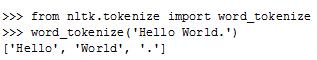
\includegraphics[scale=0.75]{static/figures/nltk3.png}
    \caption{Απομάκρυνση ανεπιθύμητων λέξεων.}
    \label{}
\end{figure}
\end{comment}
\end{itemize}

\subsection{\en {GATE for Named Entity Recognition}}
%Το σύστημα, αφού αναγνωρίσει μια ονοματισμένη οντότητα (π.χ. πρόσωπο, οργανισμό, εταιρεία κτλ.)...

Το {\en {GATE (General Architecture for Text Engineering)}} \cite{Gt01} αποτελεί πλατφόρμα ανοιχτού κώδικα για την επεξεργασία και ανάλυση κειμένων φυσικής γλώσσας, 
παρέχοντας εργαλεία ανάλυσης κειμένου. Το {\en {GATE}} διανέμεται με το σύστημα διεξαγωγής πληροφοριών γνωστό ως {\en {ANNIE}}, 
το οποίο έχει αποτελέσει τη βάση πολλών εμπορικών και ερευνητικών συστημάτων.
Το {\en {ANNIE}} είναι σε θέση να αναγνωρίσει έναν αριθμό διαφορετικών τύπων οντοτήτων, όπως ονόματα, τοποθεσίες και οργανισμούς, 
απαντώντας έτσι σε ερωτήσεις όπως “Τι συνέβη, ποιος εμπλέκεται, πότε συνέβη” κ.λπ, φράσεις οι οποίες 
ενδέχεται να κεντρίζουν το ενδιαφέρον αρκετών χρηστών ως προς την επιλογή άρθρων προς ανάγνωση. \\

\begin{figure}[!ht] \centering
\centerline{
    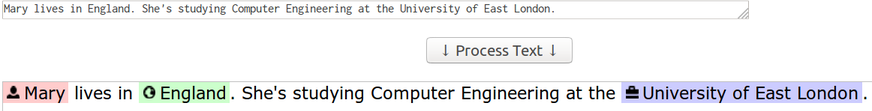
\includegraphics[scale=0.5]{static/figures/gate.png}}
    \caption{Αναγνώριση ονοματισμένων οντοτήτων.}
    \label{}
\end{figure}

\newpage

\begin{figure}[!ht] \centering
\centerline{
    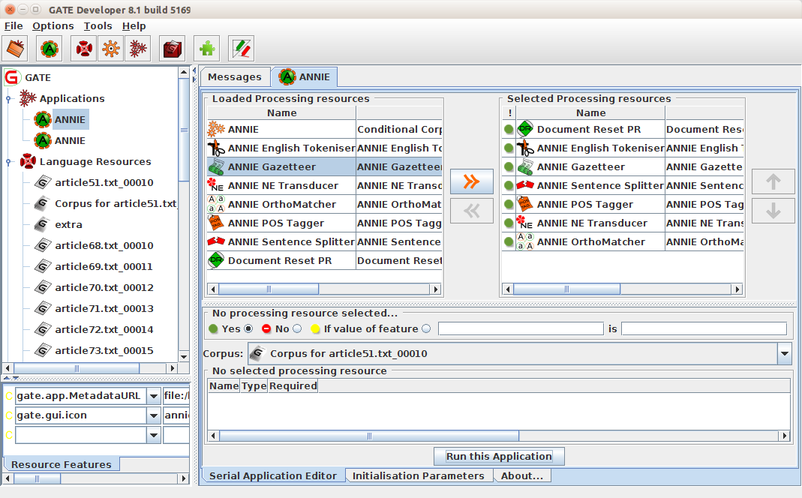
\includegraphics[scale=0.5]{static/figures/gate1.png}}
    \caption{Εφαρμογή του εργαλείου {\en {ANNIE Gazetteer}} στο {\en {corpus}} κειμένων.}
    \label{}
\end{figure}

\begin{figure}[!ht] \centering
\centerline{
    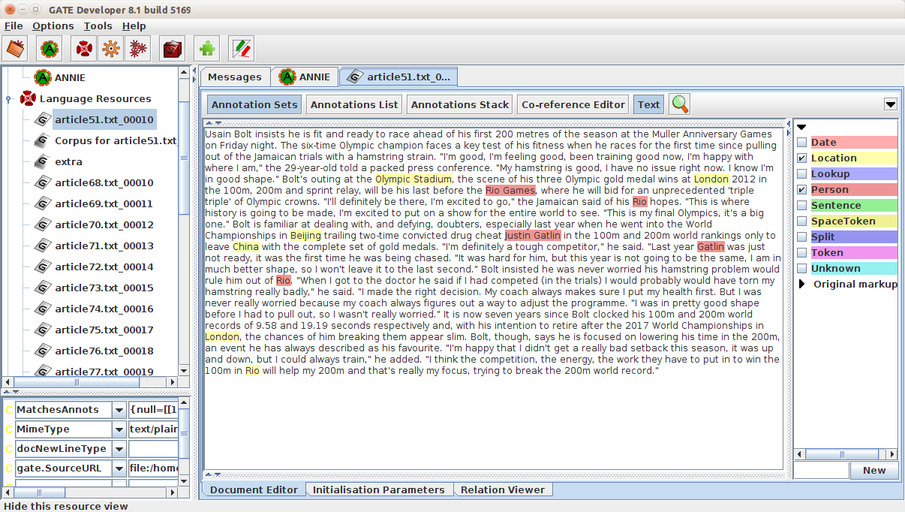
\includegraphics[scale=0.45]{static/figures/gate2.png}}
    \caption{Επιλογή των ετικετών που μας ενδιαφέρουν μέσω της δεξιάς στήλης.}
    \label{}
\end{figure}










